\documentclass[12pt]{article}
    \usepackage{float}
    \usepackage{graphicx}
    \usepackage{svg}
    \title{Temperatures are Significantly Correlated between Successive Years on Key West}
    \author{Xiaosheng Luo}
    \date{22nd October 2018}
\begin{document}
\maketitle
Are temperatures of one year significantly correlated with the next year (successive years), across years in a given location? Using the temperature data for the Key West region in Florida over the 20th Century, the correlation value was computed between successive years and compared to a distribution of 10,000 randomly permuted time series correlations. As the measurements of successive time points are climactic variables they are not independent, making a standard p-value inappropriate. Instead, the approximate p-value was calculated by dividing the number of random sample correlations greater than the actual value by the entire sample size.
\begin{figure}[H]
	\centering
	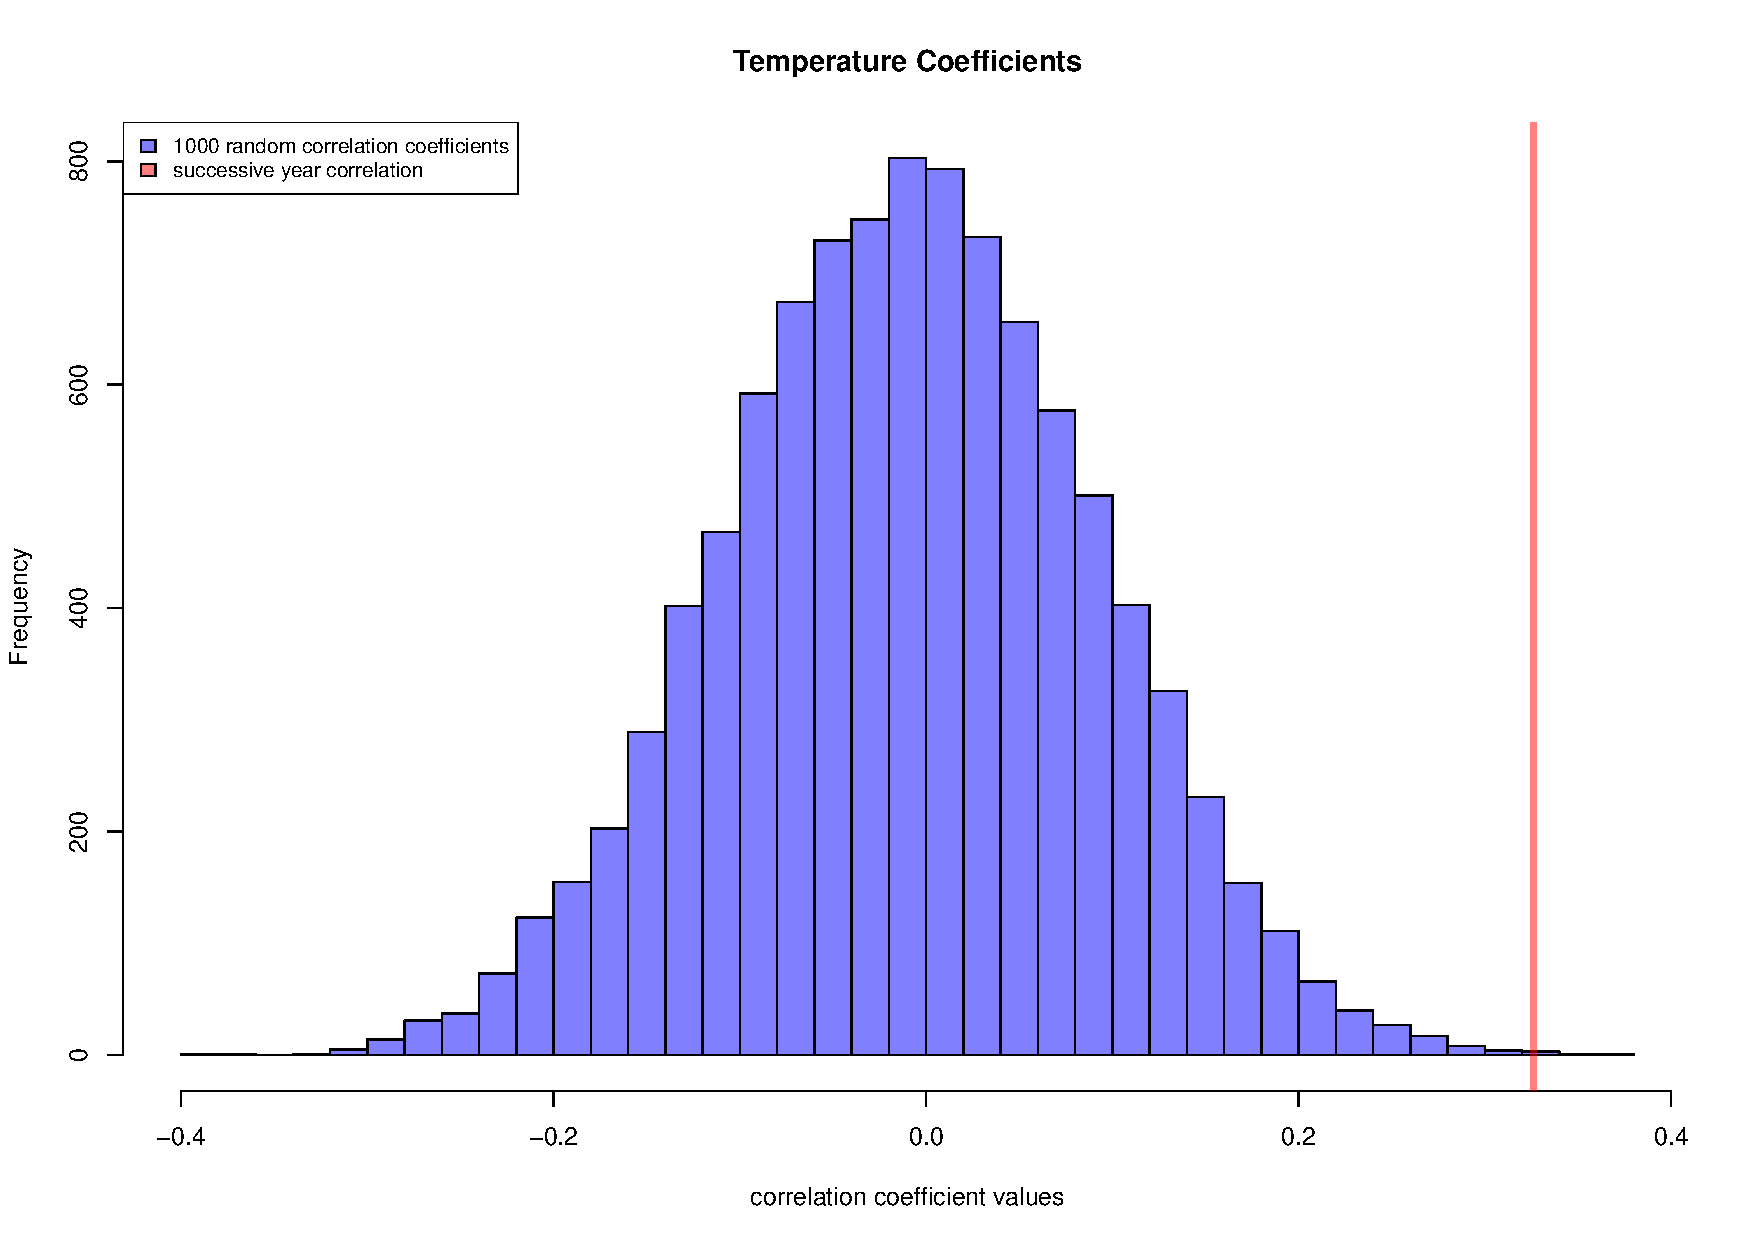
\includegraphics[scale=.3]{../results/TAutoCorr.pdf}
	\caption{Temperature Coefficient Compared between Successive Years and Rondom Years in Key West, Florida from 1901-2000.}
\end{figure}


Figure above shows a graph with a significantly positive correlation between t and t-1 years. The positive correlation shown in the graph is further backed up by a pearsons correlation value of 0.33, which was attained by computing using the $cor()$ function in R, and the p value of $~ 0.003$ indicating these results are extremely unlikely to arise by chance. Hence, it can be interpreted that one years temperature is indicative of the subsequent years temperature.

\end{document}
